\begin{frame}{Previous analysis}

\begin{itemize}
\item ``Production of $\Upsilon(1S)$ mesons from $\chi_b$ decays in $p\bar{p}$ collisions at $\sqrt{s} = 1.8\tev$'' at CDF, \hepex{9910025}.
\item ``Observation of a new $\chi_b$ state in radiative transitions to $\Upsilon(1S)$ and $\Upsilon(2S)$ at ATLAS'', \arxiv{1112.5154}
\end{itemize}
\begin{itemize}
\item ``Measurement of the fraction of $\Upsilon(1S)$ originating from $\chi_b(1P)$ in pp collisions at \sqs=7\tev'', \arxiv{1209.0282}, \intlum{32} \invpb
\item ``Observation of the $\chi_b(3P)$ state at LHCb in pp collisions at \sqs=7\tev'',
\cds{1456078}{LHCb-CONF-2012-020}, \intlum{0.9} \invfb.
\end{itemize}

\centering
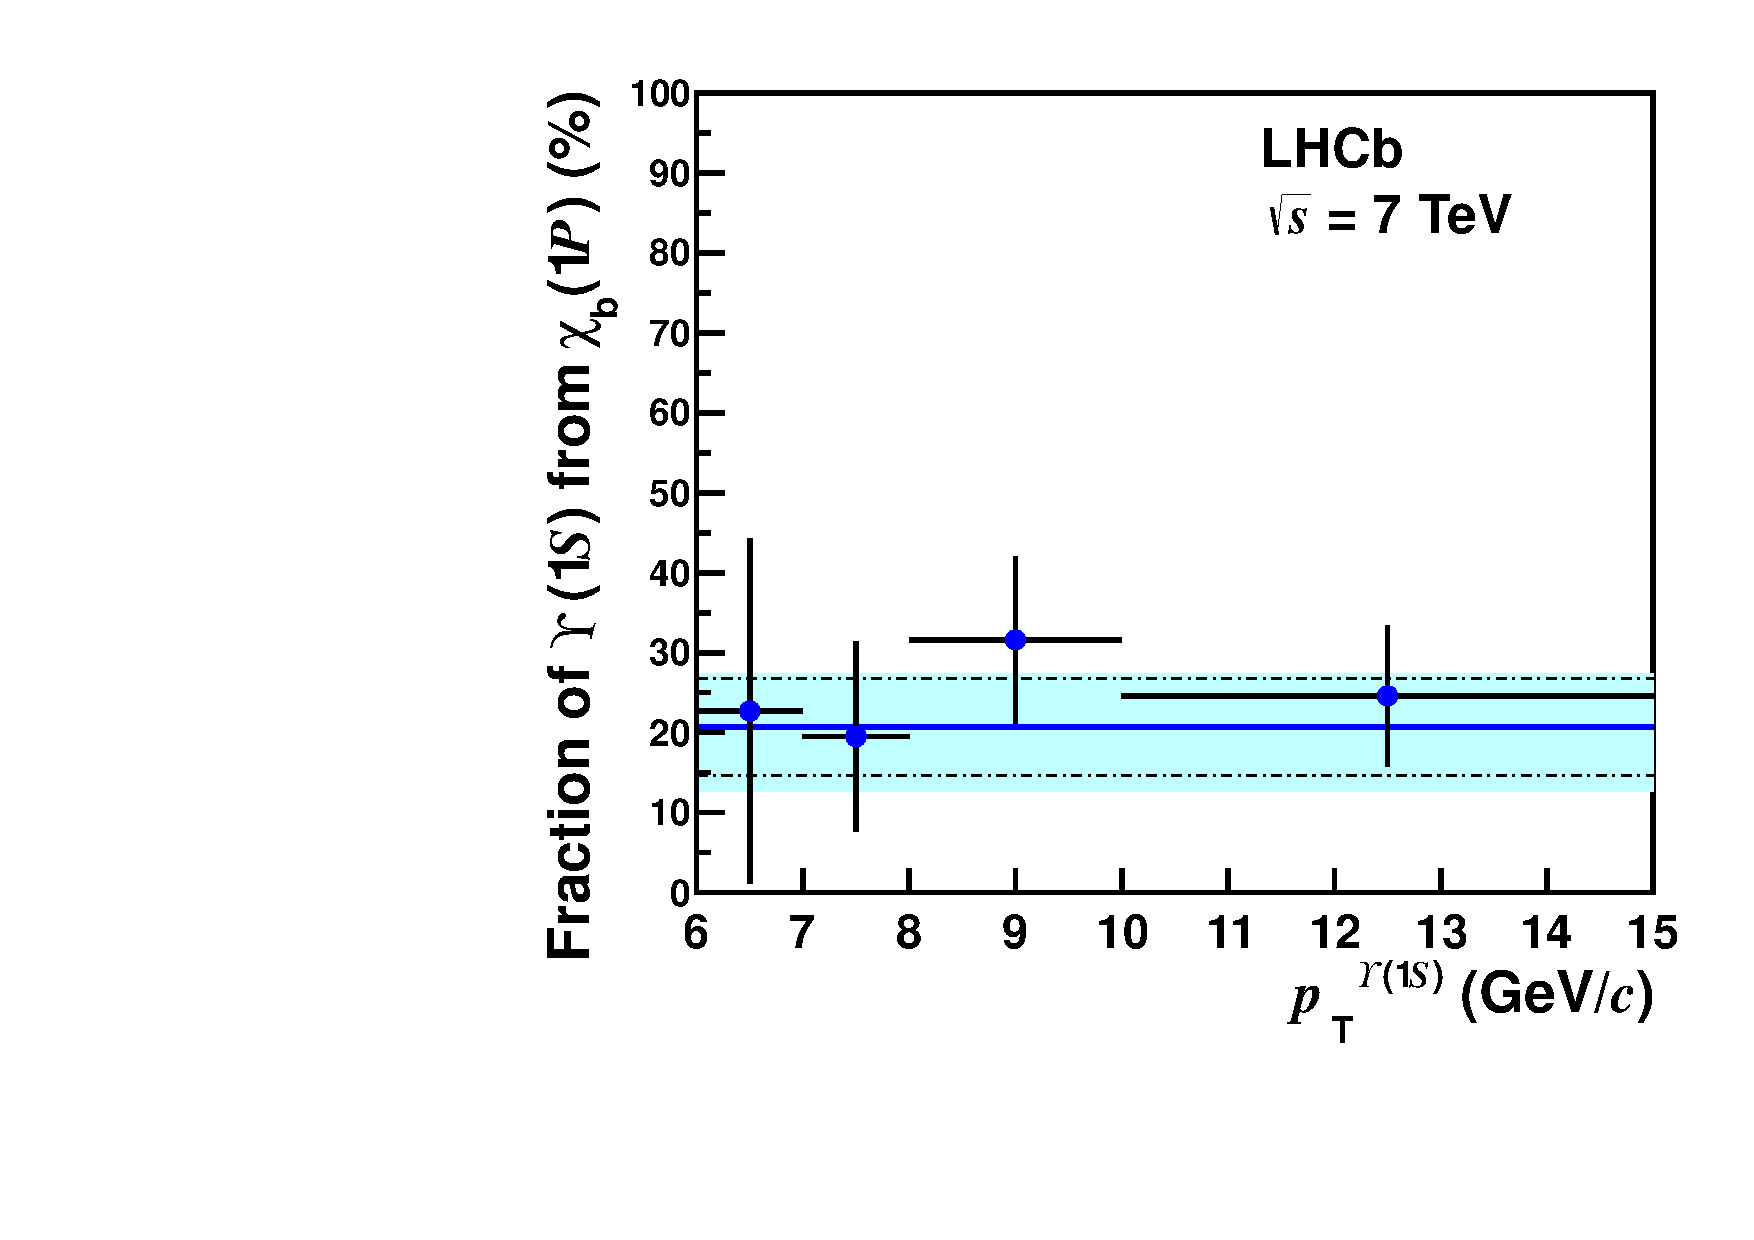
\includegraphics[width=.4\textwidth]{frac-old}
\begin{tikzpicture}
\node[anchor=south west] (image){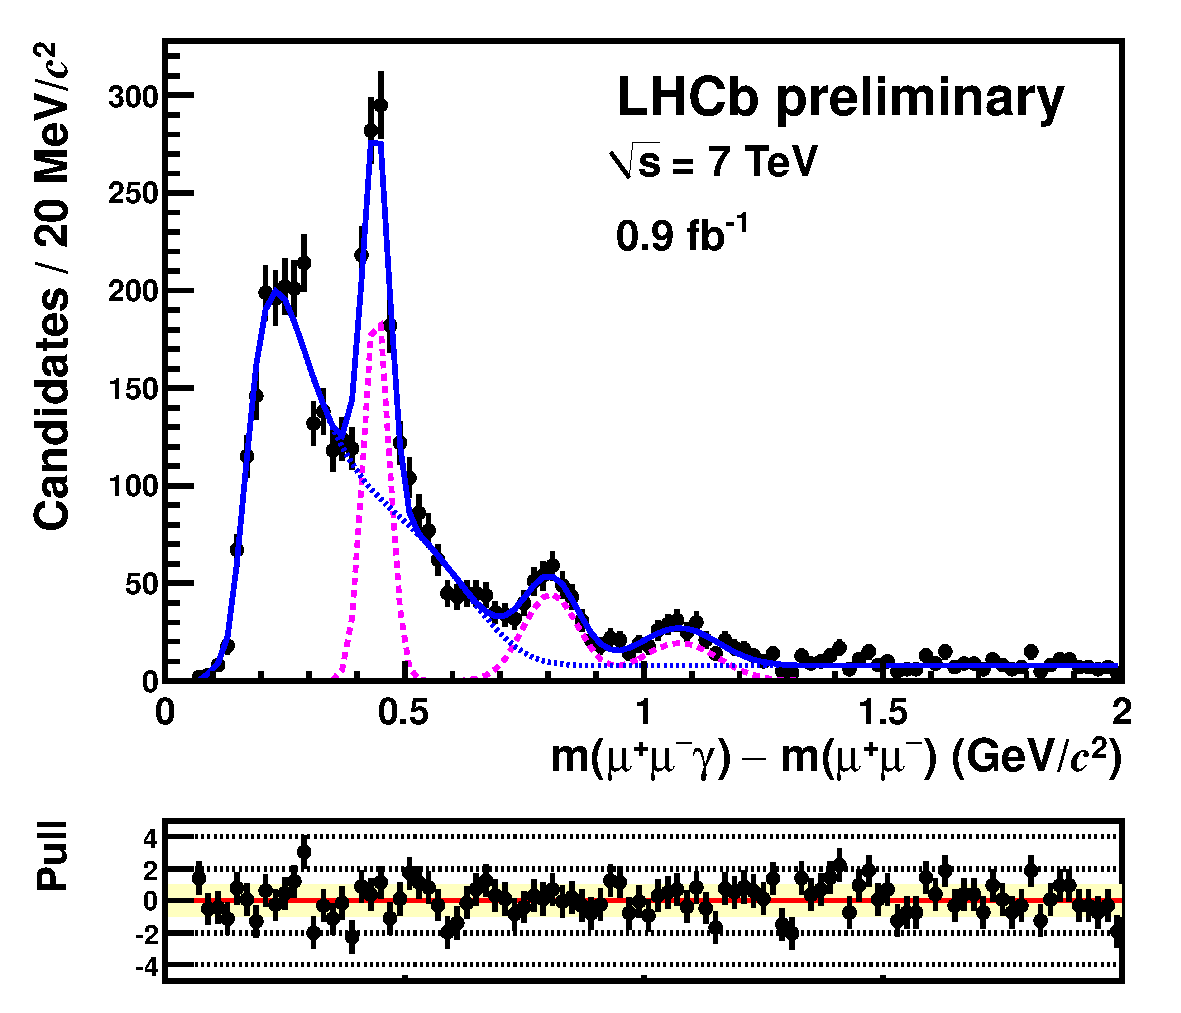
\includegraphics[width=.4\textwidth]{chib3p-old}};
\begin{scope}[x={(image.south east)},y={(image.north west)}]
    \node (cb) at (0.6,0.6) {\chibThreeP};
    \coordinate (peak) at (0.5,0.5);
    \draw [red, line width=.8pt, ->] (cb) -- (0.57,0.41);
    % \draw[help lines,xstep=.05,ystep=.05] (0,0) grid (1,1);
    % \foreach \x in {0,1,...,9} { \node [anchor=north] at (\x/10,0) {\tiny 0.\x}; }
    % \foreach \y in {0,1,...,9} { \node [anchor=east] at (0,\y/10) {\tiny 0.\y}; }
\end{scope}
\end{tikzpicture}

% \node[anchor=south east] (image2){};

\end{frame}
